
\chapter{Interpolasi Lebih Lanjut}

\section{Polinom Oskulasi}

Polinom Taylor pada Bagian \ref{sec:Taylor} dan polinom interpolasi
pada Bab \ref{chap:Interpolation} merepresentasikan dua ekstrem berlawanan
dalam spektrum polinom oskulasi. Polinom Taylor memerlukan nilai polinom
pada satu titik, sedangkan polinom interpolasi pada umumnya memerlukan
nilai polinom di beberapa titik. Polinom Taylor pada umumnya memerlukan
nilai beberapa turunan, sedangkan polinom interpolasi tidak memperbolehkan
penentuan turunan.

Himpunan polinom oskulasi mencakup polinom Taylor, polinom interpolasi,
serta bentuk-bentuk hibrida. Setiap polinom yang diharuskan melalui
sebarang himpunan titik dengan sebarang banyak turunan yang ditentukan
pada titik-titik tersebut disebut polinom oskulasi. Jadi, polinom
Taylor merupakan kasus khusus polinom oskulasi yang ditentukan oleh
satu titik dan sebarang banyak turunan pada titik tersebut. Polinom
interpolasi merupakan kasus khusus polinom oskulasi yang ditentukan
oleh sebarang banyak titik tanpa turunan pada titik mana pun. Tepatnya,
polinom oskulasi adalah polinom yang diharuskan melalui suatu himpunan
titik
\[
(t_{0},y_{0}),(t_{1},y_{1}),\ldots,(t_{n},y_{n})
\]
dengan $m_{i}$ turunan pertama yang ditentukan pada $(t_{i},y_{i})$,
$i=0,1,\ldots,n$. Seperti sebelumnya, $t_{0},t_{1},\ldots,t_{n}$
disebut simpul.

Salah satu jenis polinom oskulasi yang berguna ialah polinom Hermite,
dengan nilai polinom dan turunan pertamanya diberikan pada setiap
simpul. Secara lebih khusus lagi, polinom Hermite berderajat tiga,
atau kubik, berperan penting dalam teori aproksimasi. Karena polinom
berderajat tiga memiliki empat parameter, data---ordinat dan turunan
pertama---pada dua simpul cukup untuk menentukan polinom semacam
itu. Jadi, misalkan kita hendak mencari suatu polinom $p$ berderajat
paling tinggi tiga yang melalui $(t_{0},y_{0})$ dan $(t_{1},y_{1})$
dengan turunan $\dot{y}_{0}$ pada $t_{0}$ dan $\dot{y}_{1}$ pada
$t_{1}$.

Dengan mengingat pelajaran dari kajian kita tentang polinom interpolasi,
kita dapat memulai dengan bentuk Lagrange dari polinom interpolasi
yang melalui $(t_{0},y_{0})$ dan $(t_{1},y_{1})$ dan memikirkan
turunannya kemudian. Dengan demikian, mula-mula kita peroleh $f(t)=\frac{t-t_{1}}{t_{0}-t_{1}}y_{0}+\frac{t-t_{0}}{t_{1}-t_{0}}y_{1}$
sebagai titik awal. Tentu saja, $f$ melalui titik-titik yang disyaratkan,
tetapi polinom ini bahkan tidak mungkin kubik, dan turunannya adalah
$f'(t)=\frac{y_{0}}{t_{0}-t_{1}}+\frac{y_{1}}{t_{1}-t_{0}}$, suatu
konstanta. Alangkah baiknya jika kita dapat menambahkan padanya suatu
polinom berderajat tiga yang bernilai nol pada $t_{0}$ dan $t_{1}$
serta turunannya dapat kita kendalikan. Nah, $g(t)=(t-t_{0})(t-t_{1})^{2}$,
misalnya, bersifat kubik, bernilai nol pada $t_{0}$ dan $t_{1}$,
serta memiliki turunan $(t-t_{1})^{2}+2(t-t_{0})(t-t_{1})$, sehingga
kita setidaknya memiliki sedikit kendali atas turunannya. Baik, sekarang
mari kita cermati sedikit lebih saksama:
\[
g'(t)=(t-t_{1})^{2}+2(t-t_{0})(t-t_{1})=(t-t_{1})\left[(t-t_{1})+2(t-t_{0})\right].
\]
Jadi, $g'(t_{1})=0$ dan $g'(t_{0})=(t_{0}-t_{1})^{2}$ tidak nol.
Hal itu semestinya mengingatkan Anda pada cara kita menyusun polinom
interpolasi Lagrange. Hanya saja, di sana, nilai polinom adalah $0$
atau $1$ pada setiap simpul sebelum kita menambahkan koefisien yang
belum diketahui. Tentu saja, $\hat{g}(t)=\frac{g(t)}{(t_{0}-t_{1})^{2}}$
memiliki turunan $1$ pada $t_{1}$ dan $0$ pada $t_{0}$. Jika semuanya
digabungkan, $\hat{g}_{a}(t)=a\frac{(t-t_{0})(t-t_{1})^{2}}{(t_{0}-t_{1})^{2}}$
memiliki segala yang kita perlukan untuk mengendalikan turunan pada
$t_{0}$. Demikian pula, $\hat{h}_{b}(t)=b\frac{(t-t_{0})^{2}(t-t_{1})}{(t_{1}-t_{0})^{2}}$
memiliki segala yang kita perlukan untuk mengendalikan turunan pada
$t_{1}$. Jumlah $\hat{g}_{a}$ dan $\hat{h}_{b}$ merupakan polinom
berderajat paling tinggi tiga yang bernilai nol pada $t_{0}$ dan
$t_{1}$ serta turunannya mudah ditentukan pada $t_{0}$ dan $t_{1}$.
Akhirnya, suatu polinom $p$ berbentuk
\begin{eqnarray*}
p(t) & = & \frac{t-t_{1}}{t_{0}-t_{1}}y_{0}+\frac{t-t_{0}}{t_{1}-t_{0}}y_{1}+g_{a}(t)+h_{b}(t)\\
 &  & \frac{t-t_{1}}{t_{0}-t_{1}}y_{0}+\frac{t-t_{0}}{t_{1}-t_{0}}y_{1}+a\frac{(t-t_{0})(t-t_{1})^{2}}{(t_{0}-t_{1})^{2}}+b\frac{(t-t_{0})^{2}(t-t_{1})}{(t_{1}-t_{0})^{2}}
\end{eqnarray*}
akan menjadi polinom Hermite yang kita cari. Dua suku pertama membentuk
polinom interpolasi yang melalui titik-titik yang disyaratkan. Dua
suku terakhir bernilai nol pada $t_{0}$ dan $t_{1}$ sehingga tidak
memengaruhi interpolasi ini. Selain itu, dua suku terakhir dipilih
agar turunannya memiliki nilai yang mudah digunakan pada $t_{0}$
dan $t_{1}$. Turunan $\frac{(t-t_{1})^{2}(t-t_{0})}{(t_{0}-t_{1})^{2}}$
adalah $1$ pada $t_{0}$ dan $0$ pada $t_{1}$. Turunan $\frac{(t-t_{0})^{2}(t-t_{1})}{(t_{1}-t_{0})^{2}}$
adalah $0$ pada $t_{0}$ dan $1$ pada $t_{1}$. Ciri-ciri ini memastikan
nilai sederhana untuk $a$ dan $b$ dalam hubungannya dengan turunan
yang ditentukan. Untuk mengetahui secara tepat nilainya, tinggal kita
paksakan $\dot{p}(t_{0})=\dot{y}_{0}$ dan $\dot{p}(t_{1})=\dot{y}_{1}$:
\[
\dot{p}(x)=\frac{y_{1}-y_{0}}{t_{1}-t_{0}}+2\frac{(t-t_{1})(t-t_{0})}{(t_{0}-t_{1})^{2}}a+2\frac{(t-t_{0})(t-t_{1})}{(t_{1}-t_{0})^{2}}b+\frac{(t-t_{1})^{2}}{(t_{0}-t_{1})^{2}}a+\frac{(t-t_{0})^{2}}{(t_{1}-t_{0})^{2}}b
\]
sehingga
\[
\begin{gathered}\dot{p}(t_{0})=\frac{y_{1}-y_{0}}{t_{1}-t_{0}}+a\\
\mbox{dan}\\
\dot{p}(t_{1})=\frac{y_{1}-y_{0}}{t_{1}-t_{0}}+b.
\end{gathered}
\]
Oleh karena itu, kita memerlukan $c=\dot{y}_{0}-\frac{y_{1}-y_{0}}{t_{1}-t_{0}}$
dan $d=\dot{y}_{1}-\frac{y_{1}-y_{0}}{t_{1}-t_{0}}$. Polinom Hermite
(oskulasi) berderajat paling tinggi tiga yang diinginkan adalah 
\begin{equation}
p(t)=\frac{t-t_{1}}{t_{0}-t_{1}}y_{0}+\frac{t-t_{0}}{t_{1}-t_{0}}y_{1}+\frac{(t-t_{1})^{2}(t-t_{0})}{(t_{0}-t_{1})^{2}}(\dot{y}_{0}-m)+\frac{(t-t_{0})^{2}(t-t_{1})}{(t_{1}-t_{0})^{2}}(\dot{y}_{1}-m)\label{eq:HermiteCubicForHumans}
\end{equation}
dengan $m=\frac{y_{1}-y_{0}}{t_{1}-t_{0}}$. 

Bentuk polinom Hermite kubik ini mudah digunakan oleh manusia. Bentuk
ini bersifat formulaik dan hanya memerlukan sedikit perhitungan untuk
dituliskan. Kita akan menyebutnya bentuk Manusia dari polinom Hermite
kubik. Bentuk yang lebih ramah-komputer, yang akan kita sebut sebagai
bentuk Komputer dari polinom Hermite kubik, diperoleh melalui beda
terbagi. Secara umum, untuk polinom oskulasi dengan $k$ turunan pertama
ditentukan pada $t_{i}$, $t_{i}$ dan $y_{i}$ harus diulang $k+1$
kali dalam tabel beda terbagi. Hasil bagi yang seharusnya tidak terdefinisi
akibat pengulangan tersebut diganti dengan turunan yang ditentukan:
turunan pertama untuk beda terbagi tingkat pertama, turunan kedua
untuk beda terbagi tingkat kedua, dan seterusnya.

Untuk polinom Hermite kubik $p$ yang melalui $(t_{0},y_{0})$ dan
$(t_{1},y_{1})$ dengan turunan $\dot{y}_{0}$ pada $t_{0}$ dan $\dot{y}_{1}$
pada $t_{1}$, tabelnya tampak sebagai berikut:

\begin{center}
\begin{tabular}{ccc|c|c}
\cline{4-5}
$t_{0}$ & $y_{0}$ & $y_{0}'$ &  & \multicolumn{1}{c|}{}\tabularnewline
\cline{3-5}
$t_{0}$ & \multicolumn{1}{c|}{$y_{0}$} &  &  & \tabularnewline
\cline{3-4}
$t_{1}$ & $y_{1}$ & \multicolumn{1}{c}{$y_{1}'$} & \multicolumn{1}{c}{} & \tabularnewline
$t_{1}$ & $y_{1}$ & \multicolumn{1}{c}{} & \multicolumn{1}{c}{} & \tabularnewline
\end{tabular}
\par\end{center}

\noindent Keempat entri yang tersisa harus diisi dengan metode beda
terbagi biasa. Dapatkah Anda menghitungnya secara umum (dalam $t_{0},t_{1},y_{0},y_{1},\dot{y}_{0},\dot{y}_{1}$)?
Jawaban \vpageref{ans:hermiteCoefficients}. Dengan menggunakan hasilnya,
kita tuliskan polinom interpolasi dalam dua cara:
\begin{eqnarray*}
p(t) & = & y_{0}+\left[\dot{y}_{0}\right](t-t_{0})+\left[\frac{y_{1}-y_{0}}{(t_{1}-t_{0})^{2}}-\frac{\dot{y}_{0}}{t_{1}-t_{0}}\right](t-t_{0})^{2}\\
 &  & \qquad+\left[\frac{\dot{y}_{1}+\dot{y}_{0}}{(t_{1}-t_{0})^{2}}-2\frac{y_{1}-y_{0}}{(t_{1}-t_{0})^{3}}\right](t-t_{0})^{2}(t-t_{1})
\end{eqnarray*}
dan
\begin{eqnarray*}
p(t) & = & y_{1}+\left[\dot{y}_{1}\right](t-t_{1})+\left[\frac{\dot{y}_{1}}{t_{1}-t_{0}}-\frac{y_{1}-y_{0}}{(t_{1}-t_{0})^{2}}\right](t-t_{1})^{2}\\
 &  & \qquad+\left[\frac{\dot{y}_{1}+\dot{y}_{0}}{(t_{1}-t_{0})^{2}}-2\frac{y_{1}-y_{0}}{(t_{1}-t_{0})^{3}}\right](t-t_{1})^{2}(t-t_{0}).
\end{eqnarray*}
Seperti pada polinom interpolasi, kita memiliki dua cara untuk menentukan
polinom oskulasi Hermite kubik. Satu cara mudah bagi manusia dan cara
lainnya bagi komputer.

\subsection{Kurva B\'ezier}

Kurva B\'ezier adalah kurva parametrik dengan parameter $t\in[0,1]$
yang menghubungkan dua titik. Kurva B\'ezier paling sederhana ialah
garis lurus yang melalui kedua titik. Sebagai contoh, kurva B\'ezier
paling sederhana dari $(-1,2)$ ke $(5,-2)$ diberikan oleh fungsi
linear parametrik
\begin{eqnarray*}
x(t) & = & (1-t)(-1)+t(5)\\
y(t) & = & (1-t)(2)+t(-2),
\end{eqnarray*}
yang kita pilih untuk dituliskan dalam bentuk Lagrange. Anda dapat
memeriksa bahwa $x(0)=-1$, $x(1)=5$, $y(0)=2$, dan $y(1)=-2$.
Dengan kata lain, $x$ melalui $(0,-1)$ dan $(1,5)$ sedangkan $y$
melalui $(0,2)$ dan $(1,-2)$. Parametrisasi ini unik karena $x$
dan $y$ merupakan polinom interpolasi.

Sebaliknya, jika kita memperbolehkan $x$ dan $y$ bersifat kuadratik,
terdapat tak hingga banyak pasangan fungsi (parametrik) yang menghubungkan
$(-1,2)$ ke $(5,-2)$ bahkan jika kita mensyaratkan $x$ dan $y$
sebagai polinom interpolasi dan membatasi parameter $t$ pada interval
$[0,1]$. Hal ini bukan berarti tidak ada kurva B\'ezier kuadratik,
melainkan kita perlu menentukan lebih dari sekadar dua titik yang
akan dihubungkan. Sebagai contoh, kita dapat memilih fungsi parameternya
sebagai 
\begin{eqnarray*}
x(t) & = & a_{x}+b_{x}t+c_{x}t^{2}\\
y(t) & = & a_{y}+b_{y}t+c_{y}t^{2},
\end{eqnarray*}
yang menghasilkan enam peubah tak diketahui atau enam koefisien tak
tentu, jika Anda suka. 

Dengan memaksakan $(x(0),y(0))=(-1,2)$, kita memerlukan 
\begin{eqnarray*}
x(0) & = & a_{x}=-1\\
y(0) & = & a_{y}=2.
\end{eqnarray*}
Dengan memaksakan $(x(1),y(1))=(5,-2)$, kita memerlukan
\begin{eqnarray*}
x(1) & = & a_{x}+b_{x}+c_{x}=-1+b_{x}+c_{x}=5\\
y(1) & = & a_{y}+b_{y}+c_{y}=2+b_{y}+c_{y}=-2
\end{eqnarray*}
atau
\begin{eqnarray*}
b_{x}+c_{x} & = & 6\\
b_{y}+c_{y} & = & -4.
\end{eqnarray*}
Secara keseluruhan, kita memperoleh $a_{x}=1$, $b_{x}=6-c_{x}$,
$a_{y}=2$, dan $b_{y}=-4-c_{y}$. $c_{x}$ dan $c_{y}$ merupakan
parameter bebas, sehingga kita masih leluasa memberlakukan dua syarat
lagi pada fungsi parameter.

Setiap kurva B\'ezier kuadratik tertentu ditentukan dengan menetapkan
satu titik kontrol yang berbeda dari kedua titik ujung. Dua kurva
B\'ezier linear, satu menghubungkan $(-1,2)$ ke titik kontrol dan
yang lain menghubungkan titik kontrol ke $(5,-2)$, kemudian menentukan
kurva B\'ezier kuadratik. Misalkan $\vec{B}_{1,0}(t)$ adalah kurva
B\'ezier linear dari $(-1,2)$ ke titik kontrol dan $\vec{B}_{1,1}(t)$
adalah kurva B\'ezier linear dari titik kontrol ke $(5,-2)$. Kedua
kurva ini mendefinisikan suatu keluarga kurva B\'ezier linear, yaitu
himpunan kurva B\'ezier linear dari $\vec{B}_{1,0}(t_{0})$ ke $\vec{B}_{1,1}(t_{0})$,
dengan $t_{0}\in[0,1]$. Misalkan $\vec{B}_{2,0,t_{0}}(t)$ adalah
kurva B\'ezier linear dari $\vec{B}_{1,0}(t_{0})$ ke $\vec{B}_{1,1}(t_{0})$;
titik $\vec{B}_{2,0,t_{0}}(t_{0})$ terletak pada kurva B\'ezier
kuadratik dari $(-1,2)$ ke $(5,-2)$ melalui titik kontrol yang diberikan.
Kumpulan semua titik tersebut ketika $t_{0}$ bervariasi dari $0$
sampai $1$ merupakan kurva B\'ezier kuadratik yang kita cari. Titik
kontrol yang berbeda menentukan kuadratik yang berbeda. Sebagai contoh,
jika titik kontrolnya adalah $(0,4)$, $\vec{B}_{1,0}$ merupakan
kurva B\'ezier linear yang menghubungkan $(-1,2)$ ke $(0,4)$ dan
$\vec{B}_{1,1}$ merupakan kurva B\'ezier linear dari $(0,4)$ ke
$(5,-2$): 
\[
\begin{gathered}\vec{B}_{1,0}(t)=\left(\begin{array}{c}
(1-t)(-1)\\
(1-t)(2)+t(4)
\end{array}\right)\\
\mbox{dan}\\
\vec{B}_{1,1}(t)=\left(\begin{array}{c}
t(5)\\
(1-t)(4)+t(-2)
\end{array}\right).
\end{gathered}
\]
$\vec{B}_{2,0,t_{0}}$ adalah kurva B\'ezier linear yang menghubungkan
$\vec{B}_{1,0}(t_{0})$ ke $\vec{B}_{1,1}(t_{0})$. Oleh karena itu,
$\vec{B}_{2,0,t_{0}}(t)=(1-t)\vec{B}_{1,0}(t_{0})+t\vec{B}_{1,1}(t_{0})$
atau 
\[
\vec{B}_{2,0,t_{0}}(t)=(1-t)\left(\begin{array}{c}
(1-t_{0})(-1)\\
(1-t_{0})(2)+t_{0}(4)
\end{array}\right)+t\left(\begin{array}{c}
t_{0}(5)\\
(1-t_{0})(4)+t_{0}(-2)
\end{array}\right).
\]
Maka
\[
\vec{B}_{2,0,t_{0}}(t_{0})=(1-t_{0})\left(\begin{array}{c}
(1-t_{0})(-1)\\
(1-t_{0})(2)+t_{0}(4)
\end{array}\right)+t_{0}\left(\begin{array}{c}
t_{0}(5)\\
(1-t_{0})(4)+t_{0}(-2)
\end{array}\right).
\]
Perhatikan bahwa $\vec{B}_{2,0,t_{0}}$ bersifat kuadratik sebagai
fungsi $t_{0}$ dan bahwa $\vec{B}_{2,0,0}(0)=\begin{pmatrix}-1\\
2
\end{pmatrix}$ serta $\vec{B}_{2,0,1}(1)=\begin{pmatrix}5\\
-2
\end{pmatrix}$.

Namun, notasi $\vec{B}_{2,0,t_{0}}(t_{0})$ merepotkan, dan yang sesungguhnya
kita minati adalah parametrisasi kuadratik tersebut. Dengan menetapkan
$\vec{B}_{2,0}(t)=\vec{B}_{2,0,t}(t)$, kita memperoleh kurva B\'ezier
kuadratik dari $(-1,2)$ ke $(5,-2)$ melalui titik kontrol $(0,4)$:
\[
\vec{B}_{2,0}(t)=(1-t)\left(\begin{array}{c}
(1-t)(-1)\\
(1-t)(2)+t(4)
\end{array}\right)+t\left(\begin{array}{c}
t(5)\\
(1-t)(4)+t(-2)
\end{array}\right)
\]
dan kita memperoleh notasi yang lebih ringkas.

Dengan sedikit aljabar, ekspresi untuk $\vec{B}_{2,0}$ dapat disederhanakan,
tetapi membiarkannya tanpa penyederhanaan menegaskan asalnya. Ekspresi
tersebut merupakan hasil interpolasi linear bersarang. Kurva B\'ezier
berorde lebih tinggi dibangun dengan persarangan yang berlanjut. Sekarang
kita gunakan gagasan ini untuk mendefinisikan kurva B\'ezier dari
$\vec{P}_{0}$ ke $\vec{P_{n}}$ melalui titik-titik kontrol $\vec{P}_{1},\vec{P}_{2},\ldots,\vec{P}_{n-1}$.
Biasanya, $\vec{P}_{0}$ dan $\vec{P}_{n}$ juga dianggap sebagai
titik kontrol, sehingga kurva B\'ezier ini juga disebut sebagai kurva
B\'ezier dengan titik-titik kontrol $\vec{P}_{0},\vec{P}_{1},\ldots,\vec{P}_{n}$.
Kurva B\'ezier semacam itu akan berderajat paling tinggi $n$. 

Kita mulai dengan mendefinisikan kurva B\'ezier linear
\begin{equation}
\vec{B}_{1,i}(t)=(1-t)\vec{P}_{i}+(t)\vec{P}_{i+1},\qquad i=0,1,\ldots,n-1.\label{eq:bezierPart1}
\end{equation}
Perhatikan bahwa $\vec{B}_{1,i}$ adalah kurva B\'ezier linear dari
$\vec{P}_{i}$ ke $\vec{P}_{i+1}$. Kemudian
\begin{equation}
\vec{B}_{j,i}(t)=(1-t)\cdot\vec{B}_{j-1,i}(t)+(t)\cdot\vec{B}_{j-1,i+1}(t),\qquad j=2,3,\ldots,n;\ i=0,1,\ldots,n-j.\label{eq:bezierPart2}
\end{equation}
Perhatikan bahwa $\vec{B}_{2,i}(t)$ adalah kurva B\'ezier berderajat
paling tinggi dua yang menghubungkan $\vec{P}_{i}$ ke $\vec{P}_{i+2}$
melalui titik kontrol $\vec{P}_{i+1}$. Dengan sedikit aljabar, Anda
dapat memastikan bahwa $\vec{B}_{3,i}(t)$ berderajat paling tinggi
tiga dan menghubungkan $\vec{P}_{i}$ ke $\vec{P}_{i+3}$. Bukti induktif
akan menunjukkan bahwa $\vec{B}_{j,i}(t)$ merupakan parametrisasi
polinom berderajat paling tinggi $j$ yang menghubungkan $\vec{P_{i}}$
ke $\vec{P_{i+j}}$. Dapatkah Anda memberikan buktinya? Jawaban pada
halaman \ref{ans:bezierProof}. Dengan demikian, $\vec{B}_{n,0}(t)$
berderajat paling tinggi $n$ serta merupakan kurva B\'ezier yang
menghubungkan $\vec{P}_{0}$ ke $\vec{P}_{n}$.

Kembali ke contoh sebelumnya, kita tambahkan titik kontrol $(5,1)$
sehingga sekarang kita memiliki empat titik kontrol:
\[
\vec{P}_{0}=\begin{pmatrix}-1\\
2
\end{pmatrix},\ \vec{P}_{1}=\begin{pmatrix}0\\
4
\end{pmatrix},\ \vec{P}_{2}=\begin{pmatrix}5\\
1
\end{pmatrix},\ \vec{P}_{3}=\begin{pmatrix}5\\
-2
\end{pmatrix}.
\]
Menurut persamaan \ref{eq:bezierPart1},
\begin{eqnarray*}
\vec{B}_{1,0}(t) & = & (1-t)\vec{P}_{0}+(t)\vec{P}_{1}=(1-t)\begin{pmatrix}-1\\
2
\end{pmatrix}+t\begin{pmatrix}0\\
4
\end{pmatrix}=\begin{pmatrix}-1+t\\
2+2t
\end{pmatrix}\\
\vec{B}_{1,1}(t) & = & (1-t)\vec{P}_{1}+(t)\vec{P}_{2}=(1-t)\begin{pmatrix}0\\
4
\end{pmatrix}+t\begin{pmatrix}5\\
1
\end{pmatrix}=\begin{pmatrix}5t\\
4-3t
\end{pmatrix}\\
\vec{B}_{1,2}(t) & = & (1-t)\vec{P}_{2}+(t)\vec{P}_{3}=(1-t)\begin{pmatrix}5\\
1
\end{pmatrix}+t\begin{pmatrix}5\\
-2
\end{pmatrix}=\begin{pmatrix}5\\
1-3t
\end{pmatrix}.
\end{eqnarray*}
Dan menurut persamaan \ref{eq:bezierPart2}, 
\begin{eqnarray*}
\vec{B}_{2,0}(t) & = & (1-t)\vec{B}_{1,0}(t)+(t)\vec{B}_{1,1}(t)=(1-t)\begin{pmatrix}-1+t\\
2+2t
\end{pmatrix}+t\begin{pmatrix}5t\\
4-3t
\end{pmatrix}=\begin{pmatrix}-1+2t+4t^{2}\\
2+4t-5t^{2}
\end{pmatrix}\\
\vec{B}_{2,1}(t) & = & (1-t)\vec{B}_{1,1}(t)+(t)\vec{B}_{1,2}(t)=(1-t)\begin{pmatrix}5t\\
4-3t
\end{pmatrix}+t\begin{pmatrix}5\\
1-3t
\end{pmatrix}=\begin{pmatrix}10t-5t^{2}\\
4-6t
\end{pmatrix},
\end{eqnarray*}
serta
\begin{eqnarray}
\vec{B}_{3,0}(t) & = & (1-t)\vec{B}_{2,0}(t)+(t)\vec{B}_{2,1}(t)\nonumber \\
 & = & (1-t)\begin{pmatrix}-1+2t+4t^{2}\\
2+4t-5t^{2}
\end{pmatrix}+t\begin{pmatrix}10t-5t^{2}\\
4-6t
\end{pmatrix}\nonumber \\
 & = & \begin{pmatrix}-1+3t+12t^{2}-9t^{3}\\
2+6t-15t^{2}+5t^{3}
\end{pmatrix}.\label{eq:bezierCubicExample}
\end{eqnarray}
$\vec{B}_{3,0}(t)$ adalah kurva B\'ezier kubik dari $\begin{pmatrix}-1\\
2
\end{pmatrix}$ ke $\begin{pmatrix}5\\
-2
\end{pmatrix}$ melalui titik kontrol $\begin{pmatrix}0\\
4
\end{pmatrix}$ dan $\begin{pmatrix}5\\
1
\end{pmatrix}$. Gambar 
\begin{figure}

\caption{\label{fig:bezierViaLinearInterpolation}Tiga titik pada suatu kurva
B\'ezier kubik yang dibangun melalui interpolasi linear rekursif.}

\begin{centering}
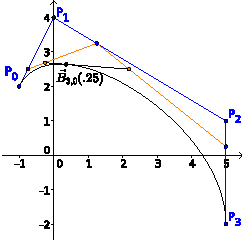
\includegraphics{figures/splines-parametric02a} 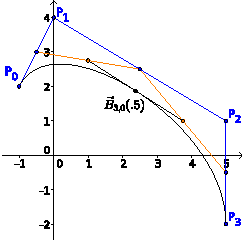
\includegraphics{figures/splines-parametric02b}
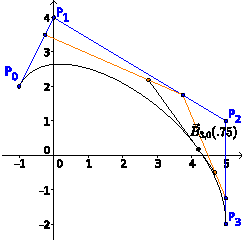
\includegraphics{figures/splines-parametric02c}
\par\end{centering}
\end{figure}
 \ref{fig:bezierViaLinearInterpolation} memperlihatkan kurva B\'ezier
ini beserta konstruksi tiga titiknya melalui interpolasi linear rekursif.
Titik-titik biru terletak di sepanjang kurva linear B\'ezier $\vec{B}_{1,0},\vec{B}_{1,1},\vec{B}_{1,2}$.
Titik-titik jingga terletak di sepanjang kurva B\'ezier kuadratik
$\vec{B}_{2,0}$ dan $\vec{B}_{2,1}$. Titik-titik hitam terletak
di sepanjang kurva B\'ezier kubik. Grafik kurva-kurva kuadratik tersebut
tidak ditampilkan agar gambar tidak menjadi terlalu rumit.

Gambar \ref{fig:bezierViaLinearInterpolation} dapat membantu Anda
memahami rekursi tersebut, tetapi yang mungkin lebih penting, membantu
Anda memahami hubungan antara titik-titik kontrol dan kurva B\'ezier.
Sebagai contoh, setelah diperiksa dengan saksama, Anda mungkin menduga
bahwa ruas garis $\vec{B}_{1,0}$ dan $\vec{B}_{1,2}$ bersinggungan
dengan kurva B\'ezier kubik $\vec{B}_{3,0}$ di $\vec{P}_{0}$ dan
$\vec{P}_{3}$, secara berturut-turut. Pemeriksaan saksama atas rumus-rumusnya
akan menegaskan hal tersebut.

Menurut rumus \ref{eq:bezierPart1} dan \ref{eq:bezierPart2}, kurva
B\'ezier berderajat paling tinggi tiga dengan titik-titik kontrol
$\vec{P}_{0},\vec{P}_{1},\vec{P}_{2},\vec{P}_{3}$ dihitung sebagai
berikut:
\begin{eqnarray*}
\vec{B}_{1,0}(t) & = & (1-t)\vec{P}_{0}+(t)\vec{P}_{1}\\
\vec{B}_{1,1}(t) & = & (1-t)\vec{P}_{1}+(t)\vec{P}_{2}\\
\vec{B}_{1,2}(t) & = & (1-t)\vec{P}_{2}+(t)\vec{P}_{3}
\end{eqnarray*}
sehingga
\begin{eqnarray*}
\vec{B}_{2,0}(t) & = & (1-t)\vec{B}_{1,0}(t)+(t)\vec{B}_{1,1}(t)=(1-t)\left[(1-t)\vec{P}_{0}+(t)\vec{P}_{1}\right]+t\left[(1-t)\vec{P}_{1}+(t)\vec{P}_{2}\right]\\
 & = & (1-t)^{2}\vec{P}_{0}+2t(1-t)\vec{P}_{1}+t^{2}\vec{P}_{2}\\
\vec{B}_{2,1}(t) & = & (1-t)\vec{B}_{1,1}(t)+(t)\vec{B}_{1,2}(t)=(1-t)\left[(1-t)\vec{P}_{1}+(t)\vec{P}_{2}\right]+t\left[(1-t)\vec{P}_{2}+(t)\vec{P}_{3}\right]\\
 & = & (1-t)^{2}\vec{P}_{1}+2t(1-t)\vec{P}_{2}+t^{2}\vec{P}_{3}
\end{eqnarray*}
sehingga
\begin{eqnarray}
\vec{B}_{3,0}(t) & = & (1-t)\vec{B}_{2,0}(t)+(t)\vec{B}_{2,1}(t)\nonumber \\
 & = & (1-t)\left[(1-t)^{2}\vec{P}_{0}+2t(1-t)\vec{P}_{1}+t^{2}\vec{P}_{2}\right]+t\left[(1-t)^{2}\vec{P}_{1}+2t(1-t)\vec{P}_{2}+t^{2}\vec{P}_{3}\right]\label{eq:bezierCubicGeneral}\\
 & = & (1-t)^{3}\vec{P}_{0}+3t(1-t)^{2}\vec{P}_{1}+3t^{2}(1-t)\vec{P_{2}}+t^{3}\vec{P}_{3}.\nonumber 
\end{eqnarray}
Dengan demikian, $\frac{d}{dt}\vec{B}_{3,0}(t)=-3(1-t)^{2}\vec{P}_{0}+3\left[(1-t)^{2}-2t(1-t)\right]\vec{P}_{1}+3\left[2t(1-t)-t^{2}\right]\vec{P}_{2}+3t^{2}\vec{P}_{3}$,
dan dari sini diperoleh
\begin{eqnarray*}
\left.\frac{d}{dt}\vec{B}_{3,0}(t)\right|_{t=0} & = & -3\vec{P}_{0}+3\vec{P}_{1}=3(\vec{P}_{1}-\vec{P}_{0})\\
\left.\frac{d}{dt}\vec{B}_{3,0}(t)\right|_{t=1} & = & -3\vec{P}_{2}+3\vec{P}_{3}=3(\vec{P}_{3}-\vec{P}_{2}).
\end{eqnarray*}
Memang, turunan $\vec{B}_{3,0}$ pada $0$ searah dengan ruas garis
dari $\vec{P}_{1}$ ke $\vec{P}_{2}$, dan turunan $\vec{B}_{3,0}$
pada $1$ searah dengan ruas garis dari $\vec{P}_{2}$ ke $\vec{P}_{3}$.
Selain itu, magnitudo turunan-turunan ini tepat tiga kali magnitudo
ruas-ruas garis tersebut.

Meskipun kita menempuh jalur yang agak berputar, kini kita melihat
cara lain untuk menghitung kurva B\'ezier kubik selain dengan menggunakan
rekursi \ref{eq:bezierPart1}/\ref{eq:bezierPart2} atau rumus \ref{eq:bezierCubicGeneral}.
Titik kontrol $\vec{P}_{0}$ dan $\vec{P}_{3}$ memberi kita dua titik
yang harus dilalui oleh $x$ dan $y$. Titik kontrol $\vec{P}_{1}$
dan $\vec{P}_{2}$ memberi kita $\dot{x}$ dan $\dot{y}$ pada kedua
titik tersebut. Dengan penentuan demikian, $x$ dan $y$ merupakan
polinom Hermite kubik! 

Tepatnya, misalkan $\vec{P}_{i}=(x_{i},y_{i})$ untuk $i=0,1,2,3$.
Maka, $x(t)$ adalah polinom Hermite kubik dengan $x(0)=x_{0}$, $\dot{x}(0)=3(x_{1}-x_{0})$,
$x(1)=x_{3}$, dan $\dot{x}(1)=3(x_{3}-x_{2})$; sedangkan $y(t)$
adalah polinom Hermite kubik dengan $y(0)=y_{0}$, $\dot{y}(0)=3(y_{1}-y_{0})$,
$y(1)=y_{3}$, dan $\dot{y}(1)=3(y_{3}-y_{2})$.

Kita tutup bagian ini dengan menghitung kurva B\'ezier dari $\begin{pmatrix}-1\\
2
\end{pmatrix}$ ke $\begin{pmatrix}5\\
-2
\end{pmatrix}$ melalui titik kontrol $\begin{pmatrix}0\\
4
\end{pmatrix}$ dan $\begin{pmatrix}5\\
1
\end{pmatrix}$ dengan menggunakan persamaan \ref{eq:HermiteCubicForHumans} dan
membandingkan hasilnya dengan \ref{eq:bezierCubicExample}. Dengan
$x(0)=-1$, $\dot{x}(0)=3$, $x(1)=5$, dan $\dot{x}(1)=0$ (dan substitusi
$x$ untuk $y$ yang dipahami), persamaan \ref{eq:HermiteCubicForHumans}
menghasilkan $m=\frac{5+1}{1-0}=6$ dan
\[
x(t)=\frac{t-1}{-1}(-1)+\frac{t}{1}(5)+\frac{(t-1)^{2}t}{1}\left(3-6\right)+\frac{t^{2}(t-1)}{1}\left(-6\right).
\]
Persamaan \ref{eq:HermiteCubicForHumans} dengan $y(0)=2$, $\dot{y}(0)=6$,
$y(1)=-2$, dan $\dot{y}(1)=-9$ menghasilkan $m=\frac{-2-2}{1-0}=-4$
dan
\[
y(t)=\frac{t-1}{-1}(2)+\frac{t}{1}(-2)+\frac{(t-1)^{2}t}{1}\left(6+4\right)+\frac{t^{2}(t-1)}{1}\left(-9+4\right).
\]
Walaupun persamaan-persamaan ini lengkap dan benar, sulit membandingkannya
dengan \ref{eq:bezierCubicExample} tanpa penyederhanaan. Dapatkah
Anda menunjukkan
\begin{eqnarray*}
x(t) & = & -1+3t+12t^{2}-9t^{3}\\
y(t) & = & 2+6t-15t^{2}+5t^{3}
\end{eqnarray*}
 sebagaimana disyaratkan? Jawaban \vpageref{ans:parametricCubics}.

\noindent\begin{digression}{Kurva B\'ezier dan CAGD}

\noindent Kurva B\'ezier pertama kali dikembangkan sekitar tahun
1960 oleh para pegawai perusahaan manufaktur otomotif Prancis. Paul
de Casteljau dari Citro\"en adalah yang pertama, tetapi Pierre B\'ezier
dari Renault memopulerkan metode ini sehingga namanya dikaitkan dengan
polinom-polinom tersebut.

Saat ini, hampir semua perangkat lunak desain grafis berbantuan komputer,
atau CAGD, menggunakan kurva B\'ezier, khususnya yang kubik, untuk
menggambar objek halus. Perangkat lunak CAGD dengan alat kurva B\'ezier
kubik akan menampilkan keempat titik kontrol dan memungkinkan pengguna
memindah-mindahkannya. Bahkan, perangkat lunak tersebut juga akan
menggambar dua kurva B\'ezier linear pada titik-titik ujung. Ini
memberi pengguna ``gagang kontrol'' untuk memanipulasi kurva. Beberapa
perangkat lunak juga akan menyertakan kurva B\'ezier linear ketiga.
Ketiga kurva linear B\'ezier tersebut bersama-sama membentuk apa
yang disebut poligon kontrol. Karena hubungan antara titik-titik kontrol
dan kurva bersifat intuitif, manipulasi titik-titik kontrol, baik
melalui gagang kontrol maupun poligon kontrol, menyediakan sarana
untuk memodelkan bentuk-bentuk halus dengan cepat. 

Namun, beberapa bentuk terlalu rumit untuk dimodelkan dengan satu
kurva B\'ezier kubik. Untuk menangani bentuk-bentuk seperti itu,
perangkat lunak CAGD memungkinkan pengguna merangkai kurva B\'ezier
kubik ujung ke ujung sehingga membentuk kurva B\'ezier komposit,
atau sepotong-sepotong, seperti yang ditampilkan di sini.

\begin{center}
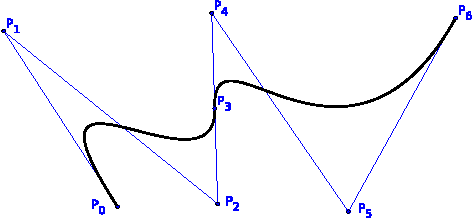
\includegraphics{figures/splines-parametric03}
\par\end{center}

\noindent Kurva ini terdiri atas dua kurva B\'ezier kubik, yang pertama
bertitik kontrol $\vec{P}_{0},\vec{P}_{1},\vec{P}_{2},\vec{P}_{3}$
dan yang kedua bertitik kontrol $\vec{P}_{3},\vec{P}_{4},\vec{P}_{5},\vec{P}_{6}$.
Karena kurva B\'ezier dimaksudkan untuk memodelkan objek halus, perangkat
lunak akan menyediakan opsi untuk memaksakan kecocokan turunan pada
titik bersama seperti $\vec{P}_{3}$. Hal ini dilakukan dengan memastikan
bahwa titik bersama berada pada ruas garis di antara dua titik kontrol
yang bersebelahan dengannya ($\vec{P}_{2}$ dan $\vec{P}_{4}$ pada
diagram ini). Anda dapat melihat versi interaktif diagram ini di \href{http://lqbrin.github.io/tea-time-numerical/ancillaries.html}{situs pendamping}.

Perangkat lunak bebas dan sumber terbuka seperti Inkscape, LibreOffice
Drawing, dan Dia menyediakan alat untuk menggambar kurva B�zier, tetapi
tidak semuanya menggunakan istilah teknis tersebut. Inkscape memiliki
alat kurva B�zier dengan nama itu, tetapi alat kurva B�zier pada LibreOffice
Drawing hanya disebut ``kurva'', sedangkan alat Dia yang hanya untuk
kurva B�zier tunggal, bukan komposit, bernama ``Bezierline''. 
\begin{description}
\item [{Referensi}] \cite{bezier,decasteljau,amsbezier,inkscape,dia,libreoffice}
\end{description}
\noindent\end{digression}

\subsection{Konsep Utama}
\begin{description}
\item [{polinom~oskulasi:}] Polinom yang grafiknya harus melalui sekumpulan
titik yang ditentukan 
\[
(x_{0},y_{0}),(x_{1},y_{1}),\ldots,(x_{n},y_{n})
\]
serta $m_{i}$ turunan pertamanya juga dapat ditentukan pada $x_{i}$.
\item [{polinom~Hermite:}] Polinom oskulasi yang harus melalui dua titik
dengan turunan pertamanya ditentukan pada setiap titik.
\item [{kurva~B\'ezier:}] Kurva yang menghubungkan dua titik melalui
polinom oskulasi parametrik.
\end{description}
\startexercises 

\subsection{Latihan}
\begin{enumerate}
\item Tentukan polinom Hermite kubik yang menginterpolasi data berikut.

\begin{center}
\begin{tabular}{c|cc}
$x$ & $f(x)$ & $f'(x)$\tabularnewline
\hline 
1 & 2 & 1\tabularnewline
5 & 3 & $-1$\tabularnewline
\end{tabular}
\par\end{center}
\item Tentukan polinom Hermite berderajat (paling tinggi) 5 yang menginterpolasi
data berikut.

\begin{center}
\begin{tabular}{c|cc}
$x$ & $f(x)$ & $f'(x)$\tabularnewline
\hline 
0 & 2 & 1\tabularnewline
$0.5$ & 2 & 0\tabularnewline
1 & 2 & 1\tabularnewline
\end{tabular}
\par\end{center}
\item Misalkan $g(x)=(\sqrt{2})^{x}$.

\begin{enumerate}
\item Dengan menggunakan $x_{0}=1$ dan $x_{1}=2$, tentukan polinom interpolasi
Hermite untuk $g$.
\item Gunakan polinom Hermite untuk menghampiri $g(1.5)$.
\item Hitung galat aktual dari hampiran ini, lalu bandingkan dengan galat
yang Anda peroleh pada soal \ref{exc:interpolation-lagrange-5} di
bagian \ref{sec:polynomialLagrange} \vpageref{exc:interpolation-lagrange-5}.
\item Polinom manakah yang menghampiri $g(1.5)$ dengan galat mutlak yang
lebih kecil, polinom Hermite atau polinom interpolasi Lagrange?
\end{enumerate}
\item Tentukan polinom yang melalui titik-titik $(0,0)$ dan $(4,-3)$ dan
yang turunannya melalui titik-titik $(0,1)$ dan $(4,1)$.
\item \label{data}Susun polinom interpolasi Hermite untuk data yang diberikan.
Lakukan ini dengan pensil, kertas dan kalkulator, atau lembar sebar.
Jangan gunakan kode Octave.

\begin{center}
\begin{tabular}{c|c|c}
$x$ & $f(x)$ & $f'(x)$\tabularnewline
\hline 
$0.1$ & $-0.29004996$ & $-2.8019975$\tabularnewline
$0.2$ & $-0.56079734$ & $-2.6159201$\tabularnewline
$0.3$ & $-0.81401972$ & $-2.4533949$\tabularnewline
\end{tabular}
\par\end{center}
\item Tentukan persamaan parametrik untuk kurva B\'ezier kubik. Ujung-ujung
``gagang kontrol'' adalah keempat titik kontrol.

\begin{center}
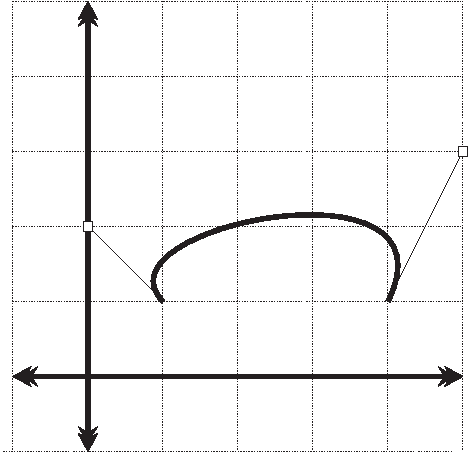
\includegraphics[scale=0.75]{figures/splines-parametric04}
\par\end{center}
\item Tuliskan persamaan parametrik kurva B\'ezier dengan titik-titik kontrol
$(-1,2)$, $(-3,2)$, $(3,1)$, dan $(3,0)$. Jawaban Anda tidak perlu
disederhanakan.
\item Susun persamaan parametrik untuk kurva B\'ezier dengan titik-titik
kontrol $(1,1),(2,1.5),(7,1.5),(6,2)$.
\item Tentukan persamaan polinom-polinom kubik yang membentuk kurva B\'ezier
komposit.

\begin{center}

\includegraphics[scale=0.6]{figures/splines-parametric06}
\par\end{center}
\item Data pada soal \ref{data} dihasilkan dengan menggunakan $f(x)=x^{2}\cos(x)-3x$.

\begin{enumerate}
\item \label{approximation}Hampiri $f(0.18)$ dengan menggunakan polinom
dari soal \ref{data}.
\item \label{error}Hitung galat mutlak dari hampiran ini.
\end{enumerate}
\item Misalkan $H(x)=x^{5}-3x^{4}+2x^{3}-6x+2$ merupakan polinom Hermite
yang menginterpolasi data

\begin{center}
\begin{tabular}{c|cc}
$x$ & $f(x)$ & $f'(x)$\tabularnewline
\hline 
0 & 2 & $-6$\tabularnewline
1 & $-4$ & \tabularnewline
2 & $-10$ & $2$\tabularnewline
\end{tabular}
\par\end{center}

diperoleh dari suatu fungsi $f$. Carilah datum yang hilang.
\item Suatu polinom Hermite $H(x)$ dikonstruksi menggunakan data

\begin{center}
\begin{tabular}{|c|c|c|c|c|}
\hline 
$x$ & $0.3$ & $0.5$ & $0.6$ & $0.8$\tabularnewline
\hline 
$f(x)$ & $0.8$ & $0.6$ & $0.3$ & $0.5$\tabularnewline
\hline 
$f'(x)$ & $1.5$ & $-1.2$ & $-5.3$ & $-2$\tabularnewline
\hline 
\end{tabular}
\par\end{center}
\begin{enumerate}
\item Carilah $(H\circ H)'(0.6)$. Dengan kata lain, carilah turunan dari
$H(H(x))$ yang dievaluasi pada $x=0.6$.
\item Carilah $(f\circ f)'(0.8)$.
\end{enumerate}
\item Polinom interpolasi Hermite untuk data berikut berbentuk $H(x)=a_{0}+a_{1}(x-0.3)+a_{2}(x-0.3)^{2}+\ldots$.

\begin{center}
\begin{tabular}{c|c|c}
$x$ & $f(x)$ & $f'(x)$\tabularnewline
\hline 
$0.30$ & $0.295$ & $-0.155$\tabularnewline
$0.32$ & $0.314$ & $-0.149$\tabularnewline
$0.35$ & $0.342$ & $-0.139$\tabularnewline
\end{tabular}
\par\end{center}
\begin{enumerate}
\item Isilah bagian yang hilang dalam bentuk $H(x)$.
\item Berapakah derajat maksimum yang mungkin untuk $H(x)$?
\item Carilah $a_{0}$ dan $a_{1}$.
\end{enumerate}
\item Konstruksikan tabel beda terbagi yang menghasilkan polinom Hermite
\[
p(x)=2-(x-1)+\frac{1}{4}(x-1)^{2}+\frac{1}{4}(x-1)^{2}(x-3).
\]
\item Kurva B\'ezier
\begin{eqnarray*}
x(t) & = & 11t^{3}-18t^{2}+3t+5\\
y(t) & = & t^{3}+1
\end{eqnarray*}
memiliki titik kontrol $(5,1)$, $(6,1)$, dan $(1,2)$. Carilah titik
kontrol keempat.
\item Berapakah jumlah minimum kurva B\'ezier kubik pada diagram tersebut,
dan mengapa?

\begin{center}

\includegraphics[scale=0.5]{figures/splines-parametric06}
\par\end{center}
\item Perhatikan grafik berikut.

\begin{center}
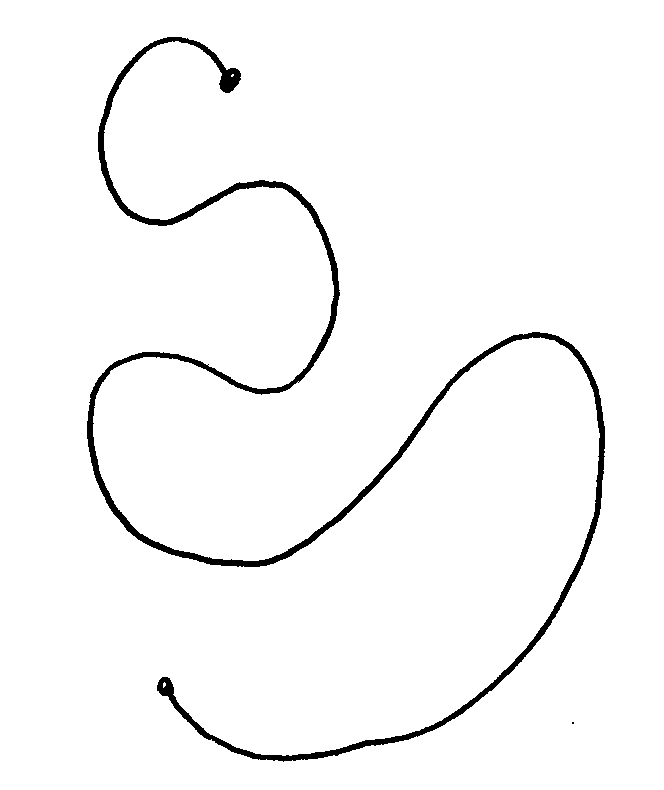
\includegraphics[scale=0.2]{figures/splines-parametric05}
\par\end{center}
\begin{enumerate}
\item Grafik tersebut tidak mungkin merupakan grafik satu kurva B\'ezier
kubik. Mengapa?
\item Grafik tersebut adalah grafik kurva B\'ezier kubik komposit. Setidaknya
berapa kurva B\'ezier kubik yang telah digabungkan, dan mengapa?
\end{enumerate}
\item Berikan tiga alasan yang dapat membuat Anda menggunakan kurva B\'ezier
alih-alih polinom Lagrange untuk memodelkan suatu grafik.
\item Polinom oskulasi $p(x)$ yang melalui $(x_{0},f(x_{0}))$ dengan $P'(x_{0})=f'(x_{0})$,
$P''(x_{0})=f''(x_{0})$, dan $P'''(x_{0})=f'''(x_{0})$ juga disebut
apa? Berikan jawaban sespesifik mungkin.
\item Kurva B\'ezier polar kubik merupakan satu-satunya fungsi polar kubik
(terparametrisasi) $(r(t),\theta(t))$ yang memenuhi data berikut.

\begin{center}
\begin{tabular}{|c|c|c|c|c|}
\hline 
$t$ & $r(t)$ & $\theta(t)$ & $\dot{r}(t)$ & $\dot{\theta(t)}$\tabularnewline
\hline 
$0$ & $r_{0}$ & $\theta_{0}$ & $\delta_{0}$ & $\mu_{0}$\tabularnewline
\hline 
$1$ & $r_{1}$ & $\theta_{1}$ & $\delta_{1}$ & $\mu_{1}$\tabularnewline
\hline 
\end{tabular}
\par\end{center}
\begin{enumerate}
\item Sebuah kurva B\'ezier kubik standar ditentukan oleh titik kontrol
$(0,0)$, $(2,0)$, $(0,1)$, dan $(0,3)$ (dalam urutan tersebut).
Konversikan data ini menjadi data koordinat polar. Ingatlah bahwa
konversi dari koordinat Kartesius ke koordinat polar melibatkan rumus
\[
r=\sqrt{x^{2}+y^{2}}\quad\mbox{dan}\quad\tan\theta=\frac{y}{x}.
\]
\item Carilah kurva B\'ezier polar kubik berdasarkan hasil Anda dari (a).
\end{enumerate}
\item \octave\ Tulislah fungsi Octave untuk menghitung polinom Hermite.
\item \octave\ Sebuah mobil yang melaju di sepanjang jalan lurus diukur
pada sejumlah titik. Data hasil pengamatan diberikan dalam tabel berikut,
dengan waktu dalam detik, jarak dalam kaki, dan kecepatan dalam kaki
per detik.

\begin{center}
\begin{tabular}{l|c|c|c|c|c}
Waktu & 0 & 3 & 5 & 8 & 13\tabularnewline
\hline 
Jarak & 0 & 225 & 383 & 623 & 993\tabularnewline
\hline 
Kecepatan & 75 & 77 & 80 & 74 & 72\tabularnewline
\end{tabular}
\par\end{center}
\begin{enumerate}
\item Hitunglah polinom interpolasi Hermite untuk data tersebut.
\item Gunakan polinom Anda dari bagian (a) untuk memprediksi posisi (jarak)
mobil dan kecepatannya pada saat $t=10$ detik.
\item Tentukan apakah mobil tersebut pernah melebihi batas kecepatan 55
mil per jam di jalan tersebut. Jika ya, kapan mobil tersebut pertama
kali melebihi kecepatan ini?
\item Berapakah prediksi kecepatan maksimum mobil tersebut?
\end{enumerate}
CATATAN: Kecepatan adalah turunan dari jarak. 
\begin{eqnarray*}
55\frac{\textrm{mil}}{\textrm{jam}} & = & 55\frac{\textrm{mil}}{\textrm{jam}}\times\frac{5280\textrm{ kaki}}{\textrm{mil}}\times\frac{1\textrm{ jam}}{3600\textrm{ detik}}\\
 & \approx & 80.67\frac{\textrm{kaki}}{\textrm{detik}}
\end{eqnarray*}

\item \octave\ Lengkapilah kode berikut.

\begin{lyxcode}
\#\#\#\#\#\#\#\#\#\#\#\#\#\#\#\#\#\#\#\#\#\#\#\#\#\#\#\#\#\#\#\#\#\#\#\#\#\#\#

\#~Written~by~Dr.~Len~Brin~~~~~~~~~~~~~\#

\#~13~March~2012~~~~~~~~~~~~~~~~~~~~~~~\#

\#~Purpose:~Evaluate~an~interpolating~~\#

\#~~~~~~polynomial~at~the~value~z.~~~~~\#

\#~INPUT:~number~z~~~~~~~~~~~~~~~~~~~~~\#

\#~~~~~~Data~x0,x1,...,xn~used~to~~~~~~\#

\#~~~~~~calculate~the~polynomial:~x~~~~\#

\#~~~~~~Entries~a0;0,~a1;0,1,~...~~~~~~\#

\#~~~~~~an;0,1,...,n~as~an~array:~c~~~~\#

\#~OUTPUT:~P(z),~the~value~of~the~~~~~~\#

\#~~~~~~interpolating~polynomial~at~z.~\#

\#\#\#\#\#\#\#\#\#\#\#\#\#\#\#\#\#\#\#\#\#\#\#\#\#\#\#\#\#\#\#\#\#\#\#\#\#\#\#

function~ans~=~divDiffEval(z,x,c)

~~n~=~length(x);

~~ans~=~c(n);

~~for~i=1:n-1

~~~~ans=(z-x(???)){*}ans+c(???);

~~end\#for

end\#function
\end{lyxcode}
\end{enumerate}
\finishexercises 

\subsection*{Jawaban}
\begin{description}
\item [{Bentuk~komputasi~polinom~Hermite:}] \label{ans:hermiteCoefficients}Empat
entri yang tersisa adalah
\begin{eqnarray*}
f_{1,1} & = & \frac{y_{1}-y_{0}}{t_{1}-t_{0}}\\
f_{0,2} & = & \frac{f_{1,1}-\dot{y}_{0}}{t_{1}-t_{0}}=\frac{y_{1}-y_{0}}{(t_{1}-t_{0})^{2}}-\frac{\dot{y}_{0}}{t_{1}-t_{0}}\\
f_{1,2} & = & \frac{\dot{y}_{1}-f_{1,1}}{t_{1}-t_{0}}=\frac{\dot{y}_{1}}{t_{1}-t_{0}}-\frac{y_{1}-y_{0}}{(t_{1}-t_{0})^{2}}\\
f_{0,3} & = & \frac{f_{1,2}-f_{0,2}}{t_{1}-t_{0}}=\frac{\dot{y}_{1}+\dot{y}_{0}}{(t_{1}-t_{0})^{2}}-2\frac{y_{1}-y_{0}}{(t_{1}-t_{0})^{3}}
\end{eqnarray*}
\item [{Kurva~B�zier~$\vec{B}_{j,i}(t)$~adalah~polinom~berderajat}] paling
tinggi $j$~yang~menghubungkan~$\vec{P_{i}}$~dengan~$\vec{P_{i+j}}$:
\label{ans:bezierProof}

\begin{proof}
Pembuktian dilakukan dengan induksi terhadap $j$, dimulai dari $j=1$:
Berdasarkan
\[
\vec{B}_{1,i}(t)=(1-t)\vec{P}_{i}+(t)\vec{P}_{i+1},\qquad i=0,1,\ldots,n-1,
\]
, berlaku $\vec{B}_{1,i}(0)=\vec{P}_{i}$ dan $B_{1,i}(1)=\vec{P}_{i+1}$,
sehingga $\vec{B}_{1,i}$ menghubungkan $\vec{P}_{i}$ dengan $\vec{P}_{i+1}$.
Selain itu, $\vec{B}_{1,i}(t)=\vec{P}_{i}+t(\vec{P}_{i+1}-\vec{P}_{i})$,
sehingga $\vec{B}_{1,i}$ merupakan polinom berderajat paling tinggi
1. Sekarang andaikan $\vec{B}_{j,i}(t)$ merupakan polinom berderajat
paling tinggi $j$ yang menghubungkan $\vec{P_{i}}$ dengan $\vec{P_{i+j}}$
untuk suatu $j\geq1$ (dan semua $i$ yang berlaku). Berdasarkan definisi,
$\vec{B}_{j+1,i}(0)=\vec{B}_{j,i}(0)$ dan $\vec{B}_{j+1,i}(1)=\vec{B}_{j,i+1}(1)$.
Berdasarkan hipotesis induksi, $\vec{B}_{j,i}(0)=\vec{P}_{i}$ dan
$\vec{B}_{j,i+1}(1)=\vec{P}_{i+j+1}$, sehingga $\vec{B}_{j+1,i}$
menghubungkan $\vec{P}_{i}$ dengan $\vec{P}_{i+j+1}$. Selain itu,
\[
\vec{B}_{j+1,i}(t)=(1-t)\cdot\vec{B}_{j,i}(t)+(t)\cdot\vec{B}_{j,i+1}(t)
\]
berderajat paling tinggi $j+1$ karena $\vec{B}_{j,i}(t)$ dan $\vec{B}_{j,i+1}(t)$
masing-masing berderajat paling tinggi $j$ (berdasarkan hipotesis
induksi). Dengan demikian, pembuktian selesai.
\end{proof}
\item [{Kurva}] B\'ezier~melalui~polinom~Hermite~kubik: \label{ans:parametricCubics}Penyederhanaannya
dapat dilakukan sebagai berikut.
\begin{eqnarray*}
x(t) & = & \frac{t-1}{-1}(-1)+\frac{t}{1}(5)+\frac{(t-1)^{2}t}{1}\left(3-6\right)+\frac{t^{2}(t-1)}{1}\left(-6\right)\\
 & = & (t-1)+5t-3t(t-1)^{2}-6t^{2}(t-1)\\
 & = & 6t-1-3t(t^{2}-2t+1)-6t^{3}+6t^{2}\\
 & = & 6t-1-3t^{3}+6t^{2}-3t-6t^{3}+6t^{2}\\
 & = & -9t^{3}+12t^{2}+3t-1
\end{eqnarray*}
dan
\begin{eqnarray*}
y(t) & = & \frac{t-1}{-1}(2)+\frac{t}{1}(-2)+\frac{(t-1)^{2}t}{1}\left(6+4\right)+\frac{t^{2}(t-1)}{1}\left(-9+4\right)\\
 & = & -2(t-1)-2t+10t(t-1)^{2}-5t^{2}(t-1)\\
 & = & -2t+2-2t+10t(t^{2}-2t+1)-5t^{3}+5t^{2}\\
 & = & 2-4t+10t^{3}-20t^{2}+10t-5t^{3}+5t^{2}\\
 & = & 5t^{3}-15t^{2}+6t+2.
\end{eqnarray*}
\end{description}

